\documentclass[11pt,a4paper]{article}
\usepackage[T1]{fontenc}
\usepackage{lmodern,amsmath,amssymb,amsthm,mathtools,booktabs,microtype,graphicx}
\usepackage[margin=25mm]{geometry}
\usepackage[hidelinks]{hyperref}

\usepackage{enumitem}
\usepackage{fancyhdr}
\pagestyle{fancy}\fancyhf{}\fancyhead[L]{Angles and Radii of the Riemann Zeros}\fancyhead[R]{Version 6}\fancyfoot[C]{\thepage}
\setlength{\headheight}{14pt}
\newtheorem{proposition}{Proposition}[section]
\theoremstyle{definition}\newtheorem{definition}[proposition]{Definition}
\theoremstyle{remark}\newtheorem{remark}[proposition]{Remark}
\newcommand{\R}{\mathbb R}\newcommand{\C}{\mathbb C}\newcommand{\Z}{\mathbb Z}

\title{Angles and Radii of the Riemann Zeros:\\ a Numerical Study of the Zeros as a Discrete Spectrum}
\author{Zeta Hoi-Ho Cheng}
\date{Version 6 --- 20 November 2026}

\begin{document}
\maketitle

\begin{abstract}
Write a nontrivial zero of $\zeta$ as $\rho=\beta+i\gamma$. Under the map $\rho\mapsto b^{\rho}$ the height $\gamma$ becomes an angle and $\beta$ a radius, and the Riemann Hypothesis becomes the statement that every image lies on one circle. We use this picture to separate, numerically and analytically, the roles of the two coordinates. A smoothed ``reverse trace'' $R(t)=-\sum_k w(\gamma_k)\cos(\gamma_k t)$ computed from the first $1200$ zeros has peaks centred at $t=\log n$ for the prime powers $n\le27$ (numerical maxima within $2.2\times10^{-4}$ of $\log n$) and none at composites; the peak heights agree with the explicit-formula prediction $\frac{\Gamma}{4\sqrt\pi}\Lambda(n)n^{-1/2}$ to within $0.01$ (an empirical agreement; a crude truncation bound is $0.1$). Perturbing the heights by a standard deviation of $1.0$ while keeping every zero on the critical line destroys this structure completely, whereas moving every zero off the line by as much as $\delta=0.49$ while keeping the heights leaves all prime-power peaks in place and produces no composite peaks. An off-line pair alters the trace only through the smooth amplitude envelope $\cosh(\delta t)$, which is $1+O(\delta^2t^2)$ at small $t$ and grows like $x^{\delta}$ at $t=\log x$; it rescales peaks but never moves them. We also record the eigenvalue-like spacing statistics of the zeros, a Landau-formula bias in their angles, and the accumulation of the Li-transformed zeros at a single point of the unit circle. The smooth background of the trace decomposes, to within $0.002$, into the contribution of the poles $s=0,1$ of the completed zeta function and the archimedean term; the poles form a pair reflected across the circle, of exactly the form an off-line zero pair would have, and Weil's positivity criterion is the statement that no further such pair exists. Finally, the projected angles fill the circle uniformly but lose both the prime bias and the eigenvalue repulsion in the limit, so that the circle retains the shape asserted by the Riemann Hypothesis while erasing the arithmetic that a proof must use. A truncated Weil quadratic form computed from primes alone is positive in every case tested; the eigenvector of its smallest eigenvalue recovers the first five ordinates of $\zeta$ to twelve digits using only the primes up to $11$, and at fixed support the smallest eigenvalue tends rapidly to $0$, so that the positivity has no margin. All theoretical statements here are classical; the paper claims no new theorem and no progress toward the Riemann Hypothesis. Its purpose is a reproducible, unified presentation of which properties of the zeros carry arithmetic information and which carry the content of the Riemann Hypothesis.
\end{abstract}

\section{Introduction}
The nontrivial zeros of the Riemann zeta function are often described as a spectrum: a discrete set of numbers that, according to the Hilbert--P\'olya philosophy, should be the eigenvalues of a natural self-adjoint or unitary operator. In the function-field case this description is a theorem. For a curve $C$ over $\mathbb F_q$ the zeros of $Z(C,T)$ are the reciprocals of the eigenvalues $\alpha_j$ of Frobenius on $H^1$, and Weil proved $|\alpha_j|=\sqrt q$: the zeros are finitely many points on a circle \cite{Weil1948}.

This paper asks a narrow question about the number-field analogue. A zero $\rho=\beta+i\gamma$ has two real coordinates. Which properties of the zeros are encoded in the heights $\gamma$, and which in the real parts $\beta$? The Riemann Hypothesis concerns only $\beta$. We show by explicit computation, and explain by the explicit formula, that the locations of the arithmetic features visible at finite scale (which integers are prime powers) are determined by the heights alone, while the real parts enter only through a smooth amplitude envelope that is close to $1$ at small scale and grows at large scale. The real parts are therefore observable at finite scale through amplitudes, but not through the location of any feature. Every ingredient is classical: the Riemann--von Mangoldt formula, the Weil explicit formula \cite{Weil1952}, Landau's formula \cite{Landau1912}, Li's criterion \cite{Li1997}, and the spacing statistics of Montgomery and Odlyzko \cite{Montgomery1973,Odlyzko1987}. The contribution is a unified geometric presentation and a set of reproducible experiments that make the separation between ``angle'' and ``radius'' quantitative.

\paragraph{Related work.} The reconstruction of prime-power lines from sums of $\cos(\gamma\log x)$ over zeros, with Gaussian smoothing, was carried out by Sakhr, Bhaduri and van Zyl \cite{SakhrBhaduriVanZyl2003}. They also moved zeros off the critical line and observed that the lines at prime powers persist with incorrect intensities, concluding that the locations depend only on the imaginary parts. Sections~\ref{sec:reverse} and~\ref{sec:angle-radius} reproduce this observation and extend it in four respects: the comparison with perturbations along the line and with a random null set, the quantitative agreement of peak heights with the explicit formula (Table~\ref{tab:heights}), the analytic form $\cosh(\delta t)$ of the off-line envelope together with the resulting finite-scale detectability of the radius, and the decomposition of the background (Table~\ref{tab:background}). The deviation of $\{\alpha\gamma\}$ from uniformity, governed by a Landau-type term that is nonzero exactly when $\alpha$ is a rational multiple of $\log p/2\pi$, was analysed by Ford and Zaharescu \cite{FordZaharescu2005} and extended in \cite{FordSoundararajanZaharescu,FordMengZaharescu}; the angle bias of Section~\ref{sec:stats} is a special case. We did not find in the literature the nearest-neighbour statistics of the wrapped angles (Table~\ref{tab:wrap}) or the reading of the poles of $\Lambda(s)$ as a maximally off-line pair in the $\alpha$-plane; both are elementary, and we make no priority claim for them.

Section~\ref{sec:pictures} describes three ways of placing the zeros on a circle. Section~\ref{sec:reverse} defines the reverse trace and checks it against the explicit formula. Section~\ref{sec:angle-radius} contains the angle--radius experiment. Section~\ref{sec:stats} records statistical properties of the angles. Section~\ref{sec:impurities} identifies the known points off the circle and relates them to Weil positivity, and Section~\ref{sec:filling} studies how the projected angles fill the circle, and Section~\ref{sec:weilform} computes a truncated Weil form from primes alone. Section~\ref{sec:discussion} discusses what the experiments imply for the search for a spectral operator, Section~\ref{sec:conclusion} summarises the helix--circle dichotomy, and Section~\ref{sec:limits} lists limitations.

\section{Three circle pictures}\label{sec:pictures}
\subsection{The critical line and its winding}
On the critical line write $\zeta(\tfrac12+it)=e^{-i\vartheta(t)}Z(t)$ with $Z$ real and $\vartheta$ the Riemann--Siegel theta function, $\vartheta(t)=\tfrac t2\log\tfrac t{2\pi}-\tfrac t2-\tfrac\pi8+O(t^{-1})$. The number of zeros with $0<\gamma\le T$ is
\begin{equation}\label{eq:RvM}
N(T)=\frac{\vartheta(T)}{\pi}+1+S(T),\qquad S(T)=\frac1\pi\arg\zeta(\tfrac12+iT).
\end{equation}
Thus zeros arise, on average, once per half-turn of the phase $\vartheta$, and the rotation speed $\vartheta'(t)\approx\frac12\log\frac t{2\pi}$ increases with height. The phase $\vartheta$ comes from the Gamma factor, that is, from the functional equation. Functions with a functional equation of the same type but no Euler product, such as the Davenport--Heilbronn function \cite{DavenportHeilbronn1936}, share this winding and nevertheless have zeros off the line. The winding explains why there are infinitely many zeros, but not where they lie.

\subsection{The Frobenius picture: angle and radius}
Fix a base $b>1$ and map a zero to $\alpha=b^{\rho}=b^{\beta}e^{i\gamma\log b}$. Its radius is $b^{\beta}$ and its angle is $\gamma\log b$. A zero lies on the critical line if and only if $\alpha$ lies on the circle $|\alpha|=\sqrt b$. The functional equation pairs $\rho$ with $1-\bar\rho$, that is, $b^{\beta}$ with $b^{1-\beta}$: an off-line zero has a partner reflected across the circle.

For a curve over $\mathbb F_q$ the natural base is $b=q$, and $Z(C,T)$ is a rational function of $T=q^{-s}$. Hence $\zeta_C(s)$ is periodic in $s$ with period $2\pi i/\log q$, there are $2g$ zeros per period, and the infinite critical line is wrapped onto the circle $|T|=q^{-1/2}$. Over $\Z$ there is no common base: the orbit lengths $\log p$ of the primes are not integer multiples of a single length. The zeros have no periodicity, and the angles $\gamma_k\log b$ for any fixed $b$ wind around the circle infinitely often. For $b=2$ the first $1200$ angles, sorted into $12$ equal sectors, give the counts
\[
57,\ 99,\ 109,\ 106,\ 113,\ 114,\ 117,\ 109,\ 108,\ 112,\ 102,\ 54,
\]
already close to uniform away from the angle $0$ (the deficit there is explained in Section~\ref{sec:stats}). The picture appropriate to $\Z$ is therefore a helix over the circle, not the circle itself: unwinding the helix gives back the critical line.

\subsection{The Li picture: one circle, one accumulation point}
Li's transformation $z=1-1/\rho$ maps the critical line onto the unit circle, the interior of the critical strip to the left of the line inside it, and the region to the right outside it. Li proved that the Riemann Hypothesis is equivalent to $\lambda_n=\sum_\rho[1-(1-1/\rho)^n]\ge0$ for all $n\ge1$ \cite{Li1997}, and Bombieri and Lagarias expressed $\lambda_n$ through the explicit formula \cite{BombieriLagarias1999}. For $\rho=\tfrac12+i\gamma$ the point $z$ lies at angular distance $2\arctan(1/(2\gamma))$ from $z=1$. The first zero sits $4.052^\circ$ from $z=1$ and the $1200$th sits $0.0348^\circ$ from it. All zeros lie on one compact circle, but the infinitely many of them accumulate at a single point. The non-compactness of the critical line has been concentrated, not removed.

\section{The reverse trace}\label{sec:reverse}
\begin{definition}
Let $\gamma_1<\gamma_2<\cdots<\gamma_K$ be the ordinates of the first $K$ zeros in the upper half-plane and $w(\gamma)=e^{-(\gamma/\Gamma)^2}$. The \emph{reverse trace} is
\[
R(t)=-\sum_{k=1}^{K}w(\gamma_k)\cos(\gamma_k t),\qquad t>0.
\]
\end{definition}
In the language of rotating phasors, each zero is a hand rotating at speed $\gamma_k$; $R(t)$ adds up the positions of the hands at time $t$. The sign is chosen so that the main features are positive.

\paragraph{Prediction from the explicit formula.} For an even test function $h$ of sufficient decay put $g(u)=\frac1{2\pi}\int_\R h(r)e^{-iru}\,dr$. The Weil explicit formula \cite{Weil1952} gives, summing over all nontrivial zeros $\rho=\tfrac12+i\gamma$ (with $\gamma\in\C$ in general),
\begin{equation}\label{eq:explicit}
\sum_{\gamma}h(\gamma)=h(\tfrac i2)+h(-\tfrac i2)-g(0)\log\pi+\frac1{2\pi}\int_\R h(r)\,\mathrm{Re}\,\frac{\Gamma'}{\Gamma}\Bigl(\frac14+\frac{ir}2\Bigr)dr-2\sum_{n\ge1}\frac{\Lambda(n)}{\sqrt n}\,g(\log n).
\end{equation}
Take $h(r)=w(r)\cos(rt)$. Then
\[
g(u)=\frac{\Gamma}{4\sqrt\pi}\Bigl(e^{-\Gamma^2(u-t)^2/4}+e^{-\Gamma^2(u+t)^2/4}\Bigr),
\]
and since $h$ is even, $R(t)=-\tfrac12\sum_\gamma h(\gamma)$ up to truncation at $K$ zeros. The prime sum therefore contributes to $R$ a Gaussian of height
\begin{equation}\label{eq:height}
A\,\frac{\Lambda(n)}{\sqrt n},\qquad A=\frac{\Gamma}{4\sqrt\pi},
\end{equation}
and width of order $\Gamma^{-1}$ centred at each $t=\log n$; the remaining terms of \eqref{eq:explicit} are smooth in $t$ and form a slowly varying background. Only prime powers can appear, since $\Lambda(n)=0$ otherwise.

\paragraph{Computation.} We take $K=1200$ (so $\gamma_K=1648.27$) and $\Gamma=600$; $A=84.628$. The weight of the last zero kept is $w(\gamma_K)<6\times10^{-4}$, but the relevant quantity is the total weight of the omitted zeros. Integrating $w$ against the zero density $\frac1{2\pi}\log\frac{\gamma}{2\pi}$ beyond $\gamma_K$ gives approximately $0.049$. Hence truncation changes $R(t)$ by at most about $0.05$, and a peak-minus-background difference by at most about $0.1$. Figure~\ref{fig:reverse} shows $R$ on $0.5\le t\le3.3$. The explicit formula centres a Gaussian of width of order $\Gamma^{-1}$ at each $t=\log p^k$; on the computational grid (step $5\times10^{-4}$) the local maxima of $R$ above the background lie within $2.2\times10^{-4}$ of $\log n$, the small offsets coming from the sloping background and neighbouring peaks. They occur for
\[
n=2,3,4,5,7,8,9,11,13,16,17,19,23,25,27,
\]
which are exactly the prime powers up to $27$. At the composites $6,10,12,14,15,18,20,21,22,24,26$ the trace equals the background, between $-1.2$ and $-2.6$. Table~\ref{tab:heights} compares the height of each peak above its local background (the mean of $R(\log n\pm0.02)$) with \eqref{eq:height}. For every $n\le27$ the discrepancy is at most $0.01$; at the composites both quantities are $0.00$. This agreement is better than the crude truncation bound of about $0.1$ guarantees, presumably because the omitted terms oscillate and largely cancel in the difference; it should be read as empirical confirmation of the normalisation of \eqref{eq:height}, not as a certified error bound.

\begin{figure}[t]
\centering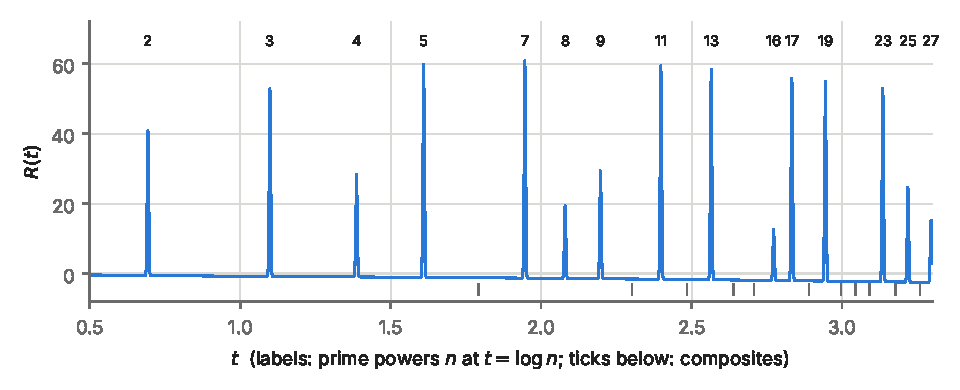
\includegraphics[width=\textwidth]{figures/fig1_reverse_trace.pdf}
\caption{Reverse trace $R(t)$ from the first $1200$ zeros, $\Gamma=600$. Labels mark prime powers $n$ at $t=\log n$; short ticks below the axis mark composites.}\label{fig:reverse}
\end{figure}

\begin{table}[t]
\centering\small
\begin{tabular}{rrrr@{\quad}rrrr}
\toprule
$n$ & observed & predicted & base & $n$ & observed & predicted & base\\
\midrule
2 & 41.47 & 41.48 & $-0.59$ & 11 & 61.18 & 61.19 & $-1.65$\\
3 & 53.67 & 53.68 & $-0.83$ & 13 & 60.19 & 60.20 & $-1.80$\\
4 & 29.33 & 29.33 & $-0.98$ & 16 & 14.66 & 14.66 & $-2.00$\\
5 & 60.90 & 60.91 & $-1.11$ & 17 & 58.15 & 58.15 & $-2.06$\\
7 & 62.23 & 62.24 & $-1.32$ & 19 & 57.16 & 57.17 & $-2.18$\\
8 & 20.74 & 20.74 & $-1.41$ & 23 & 55.32 & 55.33 & $-2.40$\\
9 & 30.99 & 30.99 & $-1.50$ & 25 & 27.24 & 27.24 & $-2.50$\\
 & & & & 27 & 17.89 & 17.89 & $-2.60$\\
\bottomrule
\end{tabular}
\caption{Peak height of $R$ above the local background at $t=\log n$ versus the explicit-formula value $A\Lambda(n)/\sqrt n$, $A=84.628$; ``base'' is the local background. At every composite $n\le27$ both columns are $0.00$.}\label{tab:heights}
\end{table}

\begin{remark}
The reverse trace is the explicit formula read from the zero side. That the zeros ``hear'' the primes in this sense goes back to Riemann and von Mangoldt, and the computation above is a quantitative illustration, not a discovery. Two features are worth isolating for what follows. First, composites are absent automatically: the operation that recovers arithmetic from the zeros sees only prime powers, each as a closed ``orbit'' of length $\log p^k$ with weight $\log p\cdot p^{-k/2}$. Second, \eqref{eq:explicit} holds unconditionally; its derivation does not use the Riemann Hypothesis.
\end{remark}

\section{Angle versus radius}\label{sec:angle-radius}
We now modify the zeros in two independent ways and recompute $R$ on $0.5\le t\le4.5$, which contains $t=\log n$ for $n\le90$. There are $34$ prime powers and $55$ composites in $2\le n\le 90$. For each modified trace we report the correlation with the ideal spike train $\sum_{n\le90}\Lambda(n)n^{-1/2}e^{-\Gamma^2(t-\log n)^2/4}$, the number of prime powers detected as local maxima within $0.004$ of $\log n$ above a threshold of one quarter of the median peak height at $n=2,3,5,7$, the number of composites so detected, and the number of stray peaks near no $\log n$.

\paragraph{Modifying the angle.} Keep every zero on the critical line and replace $\gamma_k$ by $\gamma_k+\varepsilon_k$ with independent $\varepsilon_k\sim N(0,\sigma^2)$.

\paragraph{Modifying the radius.} Keep $\gamma_k$ and move each zero to $\tfrac12\pm\delta_k+i\gamma_k$, as a pair symmetric under the functional equation. The pair contributes $e^{\delta_k t}+e^{-\delta_k t}$ times $\cos(\gamma_k t)$ to $\sum_\rho e^{(\rho-1/2)t}$ in place of $2\cos(\gamma_k t)$, so after normalisation
\[
R_\delta(t)=-\sum_k w(\gamma_k)\cosh(\delta_k t)\cos(\gamma_k t).
\]
This is a formal manipulation of the zero set, not the zero set of any known $L$-function; it isolates the effect of $\beta$ while holding $\gamma$ fixed.

\paragraph{Null comparison.} Replace the heights by $1200$ independent uniform points on $[\gamma_1,\gamma_K]$, all on the line.

\begin{table}[t]
\centering\small
\begin{tabular}{lrrrr}
\toprule
configuration & corr. & prime powers & composites & stray\\
\midrule
true zeros & 0.989 & 30/34 & 0/55 & 0\\
\addlinespace
on line, heights jittered, $\sigma=0.01$ & 0.989 & 30/34 & 0/55 & 0\\
on line, heights jittered, $\sigma=0.05$ & 0.973 & 30/34 & 0/55 & 0\\
on line, heights jittered, $\sigma=0.2$ & 0.813 & 28/34 & 1/55 & 0\\
on line, heights jittered, $\sigma=1.0$ & 0.045 & 19/34 & 31/55 & 171\\
\addlinespace
heights kept, all zeros off line, $\delta=0.05$ & 0.989 & 30/34 & 0/55 & 0\\
heights kept, all zeros off line, $\delta=0.1$ & 0.989 & 30/34 & 0/55 & 0\\
heights kept, all zeros off line, $\delta=0.25$ & 0.979 & 31/34 & 0/55 & 0\\
heights kept, all zeros off line, $\delta=0.49$ & 0.921 & 33/34 & 0/55 & 0\\
heights kept, 10\% of zeros off line, $\delta=0.45$ & 0.912 & 31/34 & 0/55 & 0\\
\addlinespace
null: random heights on the line & $-0.028$ & 16/34 & 29/55 & 210\\
\bottomrule
\end{tabular}
\caption{Angle--radius experiment on $0.5\le t\le4.5$ ($n\le90$), first $1200$ zeros, $\Gamma=600$, random seed $0$. The four prime powers missed by the unmodified trace lie near $n=90$, where the peaks fall below the detection threshold.}\label{tab:angle-radius}
\end{table}

\begin{figure}[t]
\centering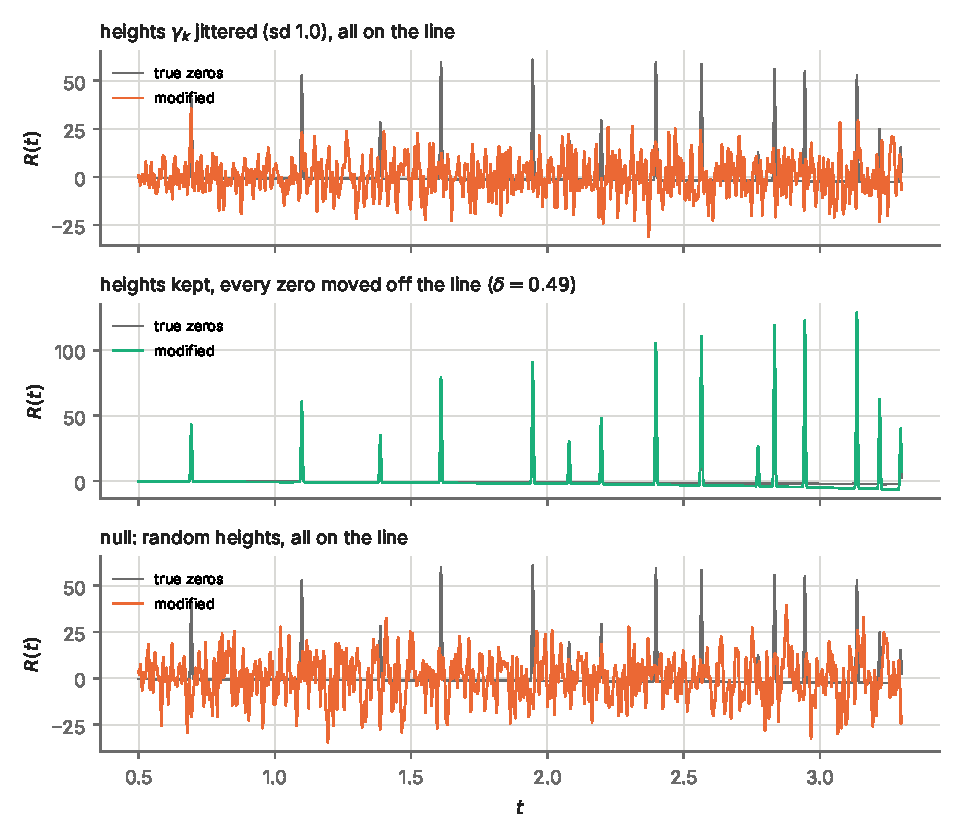
\includegraphics[width=\textwidth]{figures/fig2_angle_vs_radius.pdf}
\caption{Reverse traces of modified zero sets (colour) against the true trace (grey). Top: heights jittered with $\sigma=1.0$, all zeros on the line. Middle: heights kept, every zero moved off the line by $\delta=0.49$. Bottom: random heights on the line.}\label{fig:angle-radius}
\end{figure}

Table~\ref{tab:angle-radius} and Figure~\ref{fig:angle-radius} show the outcome. The arithmetic structure is robust to large changes of the radius and fragile under changes of the angle. Jitter of size $0.2$ begins to degrade it and jitter of size $1.0$ reduces the trace to noise comparable to the null comparison. Moving every zero almost to the edge of the critical strip changes neither the location of any peak nor the absence of composite peaks; the correlation decreases only because the peak heights acquire the envelope $\cosh(\delta t)$. The null comparison shows that placing points on the line, with the correct density, carries no arithmetic information by itself.

\paragraph{Where the radius matters.} The envelope of an off-line pair at $t=\log x$ is $\cosh(\delta\log x)\sim\tfrac12x^{\delta}$. For $\delta=0.1$ it equals $1.108$ at $x=10^2$, $2.116$ at $x=10^6$, $7.956$ at $x=10^{12}$ and $125.6$ at $x=10^{24}$. Within the window $t\le4.5$ of Table~\ref{tab:angle-radius} it never exceeds $\cosh(0.49\cdot4.5)\approx4.6$ and only rescales the peaks. Comparing one off-line term with one on-line term only suggests what happens as $x\to\infty$; with infinitely many zeros, cancellation must be controlled. The rigorous statements are classical: von Koch proved that the Riemann Hypothesis is equivalent to $\psi(x)=x+O(\sqrt x\log^2x)$ \cite{vonKoch1901}, and Landau proved that if $\Theta=\sup\beta$ then $\psi(x)-x=\Omega_\pm(x^{\Theta-\varepsilon})$ for every $\varepsilon>0$ \cite{Ingham1932}. In this sense the Riemann Hypothesis is a statement about the absence of growing envelopes at infinite length, and not about which integers are prime.

\paragraph{The radius is observable at finite scale, through amplitudes.} The envelope does not move any peak, but it does change peak heights by the factor $\cosh(\delta\log n)$. For $\delta=0.1$ this factor is $1.0024$ at $n=2$ and $1.0548$ at $n=27$; the latter would change the height $17.89$ in Table~\ref{tab:heights} by about $1$, two orders of magnitude more than the observed discrepancy. Amplitude data at finite scale can therefore detect a radius deviation of a given size within the range of zeros used. What they cannot do is exclude every $\delta>0$, since $\cosh(\delta\log n)\to1$ uniformly on any bounded range of $n$ as $\delta\to0$, nor say anything about zeros beyond the range used.

\section{Statistics of the angles}\label{sec:stats}
\paragraph{Repulsion.} Unfold the heights by $\vartheta(\gamma)/\pi$ from \eqref{eq:RvM}; the $1199$ unfolded spacings have mean $1.0001$ and minimum $0.1376$. Table~\ref{tab:spacing} and Figure~\ref{fig:stats} (left) compare the empirical distribution with independent points (Poisson) and with the Wigner surmise for eigenvalues of random unitary matrices (GUE). The zeros repel as eigenvalues do; at this low height the repulsion is even somewhat stronger than the surmise, a known finite-height effect. This is the phenomenon discovered by Montgomery and Odlyzko \cite{Montgomery1973,Odlyzko1987}; in the function-field setting Katz and Sarnak proved that the corresponding statistics arise from Frobenius \cite{KatzSarnak1999}.

\begin{table}[ht]
\centering
\begin{tabular}{lrrr}
\toprule
fraction of spacings below & zeros & Poisson & GUE surmise\\
\midrule
$0.1$ & 0.0000 & 0.0952 & 0.0011\\
$0.25$ & 0.0067 & 0.2212 & 0.0161\\
$0.5$ & 0.0742 & 0.3935 & 0.1120\\
\bottomrule
\end{tabular}
\caption{Normalised nearest-neighbour spacings of the first $1200$ zeros.}\label{tab:spacing}
\end{table}

\begin{figure}[t]
\centering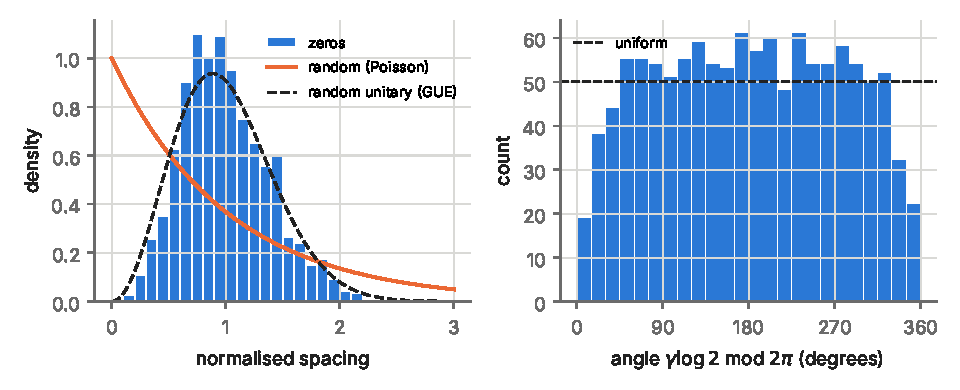
\includegraphics[width=\textwidth]{figures/fig3_statistics.pdf}
\caption{Left: normalised spacings of the first $1200$ zeros against Poisson and the GUE surmise. Right: angles $\gamma_k\log2\bmod 2\pi$ in $24$ sectors; the dashed line is the uniform count.}\label{fig:stats}
\end{figure}

\paragraph{The angles know the primes.} The deficit near angle $0$ in Section~\ref{sec:pictures} (Figure~\ref{fig:stats}, right) is predicted by Landau's formula \cite{Landau1912}: for fixed $x>1$,
\[
\sum_{0<\gamma\le T}x^{\rho}=-\frac{T}{2\pi}\Lambda(x)+O(\log T),
\]
with $\Lambda(x)=0$ unless $x$ is a prime power. On the critical line this gives the mean
\[
\frac1{N(T)}\sum_{0<\gamma\le T}\cos(\gamma\log x)\approx-\frac{T\Lambda(x)}{2\pi\sqrt x\,N(T)}.
\]
With $T=\gamma_{1200}$ and $N(T)=1200$:

\begin{center}\small
\begin{tabular}{l@{\quad}r@{\quad}r@{\quad}r@{\quad}r@{\quad}r@{\quad}r@{\quad}r}
\toprule
$x$ & 2 & 3 & 4 & 5 & 6 & 10 & 12\\
\midrule
mean of $\cos(\gamma\log x)$ & $-0.1075$ & $-0.1376$ & $-0.0752$ & $-0.1564$ & $0.0015$ & $0.0023$ & $0.0025$\\
Landau prediction & $-0.1071$ & $-0.1387$ & $-0.0758$ & $-0.1573$ & $0$ & $0$ & $0$\\
\bottomrule
\end{tabular}
\end{center}

\noindent Choosing $b=2$ in the Frobenius picture therefore produces angles that avoid $0$, because $2$ is prime; the same holds for any prime power base and fails for composite bases. This is a special case of the results of Ford and Zaharescu on the lower-order term in the distribution of $\{\alpha\gamma\}$ \cite{FordZaharescu2005}, which is nonzero precisely when $\alpha$ is a rational multiple of $\log p/2\pi$.

\section{Known impurities and positivity}\label{sec:impurities}
\paragraph{The background of the reverse trace.} Figure~\ref{fig:reverse} has, besides the prime-power peaks, a smooth background falling from about $-0.6$ to $-2.6$. By \eqref{eq:explicit} it consists of two terms: the pole term $-\tfrac12[h(\tfrac i2)+h(-\tfrac i2)]=-e^{1/(4\Gamma^2)}\cosh(t/2)$, and the archimedean term $-\frac1{4\pi}\int_\R w(r)\cos(rt)\,\mathrm{Re}\,\frac{\Gamma'}{\Gamma}(\frac14+\frac{ir}2)\,dr$ (the $\log\pi$ term is negligible for $t\ge0.5$). Table~\ref{tab:background} compares their sum with the observed background, computed as in Table~\ref{tab:heights}.

\begin{table}[ht]
\centering\small
\begin{tabular}{rrrrr}
\toprule
$n$ & observed background & pole term & archimedean term & sum\\
\midrule
2 & $-0.587$ & $-1.061$ & $0.471$ & $-0.589$\\
6 & $-1.219$ & $-1.429$ & $0.210$ & $-1.219$\\
12 & $-1.731$ & $-1.876$ & $0.145$ & $-1.731$\\
27 & $-2.597$ & $-2.694$ & $0.096$ & $-2.598$\\
\bottomrule
\end{tabular}
\caption{Decomposition of the background of $R$ at $t=\log n$. The archimedean integral is evaluated by the trapezoidal rule on $0\le r\le3000$ with step $0.02$.}\label{tab:background}
\end{table}

\paragraph{The impurities as points.} In the Frobenius picture the pole term has a geometric meaning. The completed function $\Lambda(s)=\pi^{-s/2}\Gamma(s/2)\zeta(s)$ has poles at $s=0$ and $s=1$, whose images $b^0=1$ and $b^1=b$ lie inside and outside the circle $|\alpha|=\sqrt b$, as a pair reflected across it. In the reverse trace this pair contributes $\cosh(t/2)$, which is exactly the contribution $\cosh(\delta t)$ of an off-line pair (Section~\ref{sec:angle-radius}) with the extreme value $\delta=\tfrac12$; it is the main term $x$ of $\psi(x)$. If one works with $\zeta$ instead of $\Lambda$, the trivial zeros $s=-2,-4,\dots$ appear as a further sequence of points of radius $b^{-2n}$ converging to the centre; their contribution is the term $-\tfrac12\log(1-x^{-2})$ in von Mangoldt's formula for $\psi(x)$, and in the completed function they are absorbed by the Gamma factor, that is, by the archimedean term of Table~\ref{tab:background}. All these known points lie on the positive real axis of the $\alpha$-plane (Figure~\ref{fig:circle}). The Riemann Hypothesis is equivalent to the statement that they are the only points off the circle.

\begin{figure}[t]
\centering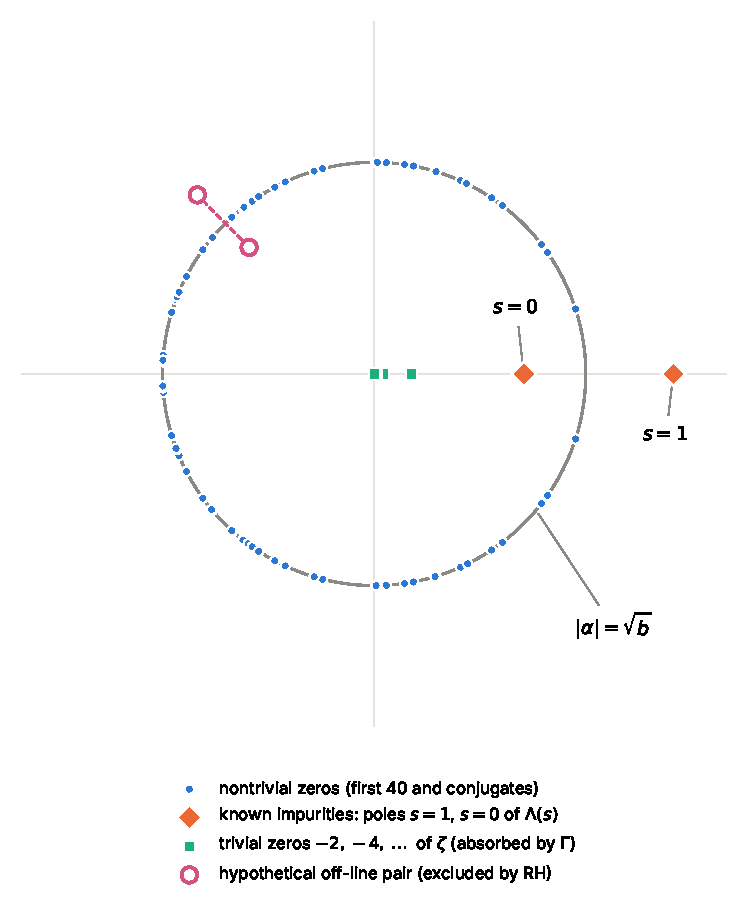
\includegraphics[width=0.72\textwidth]{figures/fig4_circle.pdf}
\caption{The $\alpha$-plane for $b=2$. Blue: the first $40$ nontrivial zeros and their conjugates, on the circle $|\alpha|=\sqrt2$. Orange: the poles $s=0,1$ of $\Lambda$. Green: trivial zeros of $\zeta$. Open circles: a hypothetical off-line pair, reflected across the circle. The sparsity of zeros near angle $0$ is the Landau bias of Section~\ref{sec:stats}.}\label{fig:circle}
\end{figure}

\paragraph{Positivity as the absence of further impurities.} We use the test class of Weil's criterion in the form given by Bombieri \cite{Bombieri2000}. Let $f$ be a smooth complex-valued function with compact support in $(0,\infty)$, put $f^*(x)=x^{-1}\overline{f(1/x)}$, and let $g=f*f^*$ be the multiplicative convolution. With the Mellin transform $F(s)=\int_0^\infty f(x)x^{s-1}\,dx$, which is entire, the Mellin transform of $g$ is
\[
H(s)=F(s)\overline{F(1-\bar s)}.
\]
Because $f$ has compact support, $H$ decays rapidly on vertical lines, the sum over zeros converges absolutely, and the prime-power sum below is finite. On the critical line $1-\bar s=s$, so $H(\tfrac12+i\gamma)=|F(\tfrac12+i\gamma)|^2\ge0$. For an off-line pair $\rho$, $\rho'=1-\bar\rho$ one finds
\[
H(\rho)+H(\rho')=2\,\mathrm{Re}\bigl(F(\rho)\overline{F(\rho')}\bigr),
\]
which is a product of values at two different points and can be made negative by a suitable choice of $f$. The explicit formula expresses the sum over zeros as
\[
\sum_\rho H(\rho)=H(0)+H(1)-P(g)-A(g),\qquad P(g)=\sum_{n\ge2}\Lambda(n)\bigl(g(n)+n^{-1}g(n^{-1})\bigr),
\]
where $A(g)$ is the archimedean term, a linear functional of $g$ given explicitly, with the precise normalisations, in \cite{Bombieri2000}; the pole contribution $H(0)+H(1)=2\,\mathrm{Re}(F(0)\overline{F(1)})$ has the same indefinite form as an off-line pair and is therefore separated out. Weil's criterion \cite{Weil1952,Bombieri2000} states that the Riemann Hypothesis holds if and only if $\sum_\rho H(\rho)\ge0$, equivalently the right-hand side is nonnegative, for every such $f$. In the language of this paper: positivity of the right-hand side, a statement about primes and the archimedean place alone, is equivalent to the absence of any impurity beyond the known pair. The function-field case has the same structure. In $Z(C,T)=P(T)/((1-T)(1-qT))$ the eigenvalues $1$ and $q$ of Frobenius on $H^0$ and $H^2$ lie off the circle $|\alpha|=\sqrt q$; Weil's proof does not remove them but projects them out, since by the Hodge index theorem the intersection pairing on $C\times C$ is definite on the orthogonal complement of the two fibre classes.

\section{Filling the circle}\label{sec:filling}
For a fixed base $b$ the angles $\gamma_k\log b\bmod2\pi$ are equidistributed on the circle \cite{Hlawka1975}. Unconditionally, Fujii bounded the discrepancy by $O(\log\log T/\log T)$ \cite{Fujii1976}; under the Riemann Hypothesis, Hlawka obtained $O(1/\log T)$, which is sharp for $\alpha$ of the form above \cite{FordSoundararajanZaharescu}. Every arc therefore eventually receives a share of zeros proportional to its length, and the set of angles is dense. It is nevertheless countable, so almost every angle is never attained exactly. Table~\ref{tab:filling} shows the approach to equidistribution for $b=2$.

\begin{table}[ht]
\centering\small
\begin{tabular}{rrrrr}
\toprule
zeros $N$ & height $T$ & largest empty arc & mean of $\cos(\gamma\log2)$ & Landau prediction\\
\midrule
40 & 122.9 & $55.6^\circ$ & $-0.2392$ & $-0.2398$\\
100 & 236.5 & $29.6^\circ$ & $-0.1743$ & $-0.1845$\\
300 & 541.8 & $10.6^\circ$ & $-0.1414$ & $-0.1409$\\
600 & 939.0 & $8.7^\circ$ & $-0.1222$ & $-0.1221$\\
1200 & 1648.3 & $2.5^\circ$ & $-0.1075$ & $-0.1071$\\
\bottomrule
\end{tabular}
\caption{Filling of the circle by the angles $\gamma_k\log2$.}\label{tab:filling}
\end{table}

The bias produced by the prime $2$ decays like $1/\log T$: by Landau's formula the mean of $\cos(\gamma\log2)$ is approximately $-\log2/(\sqrt2(\log\frac T{2\pi}-1))$, which equals $-0.0446$ at $T=10^6$, $-0.0198$ at $T=10^{12}$ and $-0.0093$ at $T=10^{24}$. It tends to $0$, consistent with equidistribution. Since the error term in Landau's formula is $O(\log T)$ while the main term is of order $T$, the bias is negative for all sufficiently large $T$; the formula alone does not exclude cancellation at particular small heights.

\paragraph{Wrapping destroys the repulsion.} Table~\ref{tab:wrap} compares normalised nearest-neighbour spacings along the line (as in Table~\ref{tab:spacing}) with those of the wrapped angles, normalised by the mean spacing $2\pi/N$. In this sample the wrapped spacings are close to Poissonian. A heuristic explanation is that neighbours on the circle typically come from distant turns of the helix and are only weakly correlated. Hlawka's theorem concerns equidistribution, a global property, and does not by itself determine local spacing statistics; the Poisson behaviour is a finite-sample observation, not a theorem. Within that limitation, the eigenvalue-like repulsion is a feature of the helix that does not survive the projection.

\begin{table}[ht]
\centering\small
\begin{tabular}{lrrr}
\toprule
fraction of spacings below & along the line & wrapped, $b=2$ & Poisson\\
\midrule
$0.1$ & 0.000 & 0.104 & 0.095\\
$0.25$ & 0.007 & 0.242 & 0.221\\
$0.5$ & 0.074 & 0.397 & 0.393\\
\bottomrule
\end{tabular}
\caption{Spacings along the critical line versus on the circle, first $1200$ zeros.}\label{tab:wrap}
\end{table}

\section{The positivity bridge, computed}\label{sec:weilform}
Section~\ref{sec:impurities} identified Weil positivity as the bridge from arithmetic to shape. Here we compute a finite version of it from primes alone, following the programme of Connes, Consani and Moscovici \cite{CCM2023,CCM2025}; a rigorously certified treatment of related truncations is given by Groskin \cite{Groskin2026}. Our computations are high-precision numerics, not interval certificates.

\paragraph{Setup.} In the logarithmic variable $u$, take even test functions supported in $[-L/2,L/2]$ with basis $\phi_k(u)=\cos(w_ku)$, $w_k=(2k+1)\pi/L$, $0\le k<N$; they vanish at the endpoints and
\[
\widehat{\phi_k}(r)=(-1)^k\cos\Bigl(\frac{rL}2\Bigr)\frac{2w_k}{w_k^2-r^2}.
\]
For $h=\widehat{\phi_j}\widehat{\phi_k}$ the function $g=\phi_j*\phi_k$ is supported in $[-L,L]$ and has a closed form. Inserting $h$ into \eqref{eq:explicit} gives the symmetric matrix
\[
Q_{jk}=2A_jA_k-g(0)\log\pi+\psi(\tfrac14)g(0)+2\int_0^\infty\frac{e^{-u/2}}{1-e^{-2u}}\bigl(g(0)-g(u)\bigr)du-2\sum_{n<e^{L}}\frac{\Lambda(n)}{\sqrt n}\,g(\log n),
\]
where $A_k=\widehat{\phi_k}(\tfrac i2)$, so that the pole term is of rank one for even test functions, and the archimedean term has been rewritten using $\mathrm{Re}\,\psi(\frac14+\frac{ir}2)=\psi(\frac14)+\int_0^\infty e^{-t/4}(1-\cos\frac{rt}2)(1-e^{-t})^{-1}dt$. No zeros enter. On the zero side the same matrix equals $2\sum_{\gamma>0}\widehat\phi(\gamma)\widehat\phi(\gamma)^{\mathsf T}$, which is positive semidefinite when all $\gamma$ are real; Weil's criterion therefore implies $Q\succeq0$ for every $L$ and $N$. All entries were computed with \texttt{mpmath} at $50$--$90$ significant digits.

\paragraph{Cross-check.} For $e^L=13$, $N=8$, Table~\ref{tab:weilcheck} compares the eigenvalues of $Q$ computed from primes with those of the zero-side matrix built from the first $1200$ zeros in double precision. They agree to three to five digits down to $4\times10^{-13}$; below that the zero-side computation reaches its precision floor. Raising the working precision of $Q$ from $50$ to $80$ digits leaves all twelve printed digits unchanged.

\begin{table}[ht]
\centering\small
\begin{tabular}{rr}
\toprule
from primes (no zeros) & from the first 1200 zeros\\
\midrule
$3.04458684$ & $3.04458683$\\
$6.82867\times10^{-2}$ & $6.82865\times10^{-2}$\\
$8.44831\times10^{-4}$ & $8.44818\times10^{-4}$\\
$1.14402\times10^{-5}$ & $1.14397\times10^{-5}$\\
$2.86287\times10^{-9}$ & $2.86246\times10^{-9}$\\
$3.92951\times10^{-13}$ & $3.92842\times10^{-13}$\\
$2.37971\times10^{-17}$ & below double precision\\
$1.26578\times10^{-22}$ & below double precision\\
\bottomrule
\end{tabular}
\caption{Eigenvalues of the truncated Weil form, $e^L=13$, $N=8$.}\label{tab:weilcheck}
\end{table}

\paragraph{The ground state locates the zeros.} Let $c$ be the eigenvector of the smallest eigenvalue and $F(r)=\sum_kc_k\widehat{\phi_k}(r)$. Discarding the common factor $\cos(rL/2)$, the real zeros of $F$ approximate the ordinates of $\zeta$. For $e^L=13$, where only the prime powers $2,3,4,5,7,8,9,11$ contribute because $g(L)=0$, the case $N=14$ gives
\[
14.1347251417,\quad21.0220396388,\quad25.0108575801,\quad30.4248761259,\quad32.9350615877,
\]
the first five ordinates to all twelve printed digits, followed by $37.58619$ against $\gamma_6=37.58618$. With $e^L=100$ and $N=16$ the first five again agree to at least ten digits. This is the phenomenon reported in \cite{CCM2023}; in the terms of this paper, the near-null direction of the positivity form is a test function whose transform vanishes at the zeros, so it carries their angles.

\paragraph{No spectral gap.} At fixed support the smallest eigenvalue decreases rapidly with $N$ (Table~\ref{tab:weilscan}), by roughly four orders of magnitude for every two added basis functions, while the recovered ordinates become more accurate.

\begin{table}[ht]
\centering\small
\begin{tabular}{rrrl}
\toprule
$N$ & smallest eigenvalue & second smallest & first three ground-state zeros\\
\midrule
4 & $6.21\times10^{-14}$ & $4.18\times10^{-9}$ & $14.13495,\ 23.86071,\ 47.68113$\\
6 & $1.70\times10^{-18}$ & $2.25\times10^{-13}$ & $14.13473,\ 21.03273,\ 25.07428$\\
8 & $1.27\times10^{-22}$ & $2.38\times10^{-17}$ & $14.13473,\ 21.02204,\ 25.01094$\\
10 & $1.12\times10^{-25}$ & $1.27\times10^{-20}$ & $14.13473,\ 21.02204,\ 25.01086$\\
12 & $6.22\times10^{-29}$ & $1.75\times10^{-23}$ & $14.13473,\ 21.02204,\ 25.01086$\\
14 & $7.00\times10^{-32}$ & $4.07\times10^{-26}$ & $14.13473,\ 21.02204,\ 25.01086$\\
\bottomrule
\end{tabular}
\caption{Truncated Weil form at fixed support $e^L=13$ as the number of basis functions grows ($90$ digits).}\label{tab:weilscan}
\end{table}

The form is thus positive on every truncation tested, but its infimum over the full space of test functions with this support appears to be $0$: there is no gap that a perturbative argument could exploit, and positivity of finite truncations does not by itself extend to the full space, as also noted in \cite{Groskin2026}. The two features are the two halves of the angle--radius picture. The directions in which the form nearly vanishes are those whose transforms vanish at the zeros, and they encode the angles; positivity in the remaining directions is the statement about the radius. A proof along this route must establish a positivity with no margin, which is why it requires exact structure rather than estimates.

\section{Discussion}\label{sec:discussion}
\paragraph{What the ``discrete circle'' is.} The experiments support the following description. The zeros form a discrete set on a helix over a circle, equivalently on the critical line, or on the Li circle with a single accumulation point. Their angles encode the prime powers with exact weights (Section~\ref{sec:reverse}), are biased by each prime as Landau's formula predicts, and repel one another along the line like the eigenvalues of a unitary operator (Section~\ref{sec:stats}); the repulsion does not survive projection onto the circle (Section~\ref{sec:filling}). Their common radius is the content of the Riemann Hypothesis. At finite scale a radius deviation $\delta$ moves no feature of the reverse trace and changes amplitudes only by $\cosh(\delta\log n)$ (Section~\ref{sec:angle-radius}).

\paragraph{Consequences for a spectral operator.} A Hilbert--P\'olya operator must reproduce all of the above. The experiments suggest a list of necessary properties for any candidate:
\begin{enumerate}[label=(\arabic*)]
\item it is defined from arithmetic data, without prior knowledge of the zeros;
\item its eigenvalue count follows the Weyl law $\frac T{2\pi}\log\frac T{2\pi}-\frac T{2\pi}+O(\log T)$;
\item its spacings exhibit GUE-type repulsion;
\item its trace formula reproduces the explicit formula \eqref{eq:explicit}, in particular the prime-power peaks of Table~\ref{tab:heights};
\item the space on which it acts carries an inner product that can be proved positive definite.
\end{enumerate}
Connes' scaling action on the ad\`ele class space \cite{Connes1999} satisfies (1) and (4), realises the zeros as a spectrum, and is consistent with (2)--(3); Meyer \cite{Meyer2005} constructed an operator on a nuclear function space whose spectrum is exactly the set of zeros, without assuming the Riemann Hypothesis. In both cases the space is not a Hilbert space on which the operator is self-adjoint or unitary, and in Connes' framework positivity of the relevant inner product is equivalent to Weil positivity, hence to the Riemann Hypothesis; Connes and Consani have proved this positivity for test functions of small support \cite{ConnesConsani2021}. Item (5) is therefore the open part. Section~\ref{sec:angle-radius} indicates why it cannot be bypassed by finite-scale data: such data locate features through the angles and constrain the radius only through amplitude factors that tend to $1$ as $\delta\to0$, whereas (5) must exclude every $\delta>0$ at every height.

\paragraph{Why integrality must enter.} Beurling's generalised primes produce zeta functions for arbitrary ``prime'' sequences, and their reverse traces have the same structure as Section~\ref{sec:reverse} with $\log p$ replaced by the logarithms of the chosen primes. Diamond, Montgomery and Vorhauer constructed such a system whose integer-counting function is very regular but whose zeta function has zeros off the line \cite{DMV2006}. Hence regularity of the angle data is not sufficient; a proof that the radius is constant must use a property of the actual integers. In the function-field case the corresponding property is the integrality of Weil numbers, which in the converse direction allows the Honda--Tate theorem to reconstruct an abelian variety from a set of points on the circle \cite{Tate1966,Honda1968}.

\section{Conclusion: helix, circle and positivity}\label{sec:conclusion}
The experiments separate two objects that are often identified.

\emph{The helix} (equivalently the critical line with its heights) carries the arithmetic. The explicit formula ties the zeros to the prime powers through an exact identity (Table~\ref{tab:heights}), Landau's formula imprints each prime on the angles (Table~\ref{tab:filling}), and the zeros repel like eigenvalues along it (Tables~\ref{tab:spacing} and~\ref{tab:wrap}). These laws are global: they constrain sums over all zeros, while no formula is known for an individual height $\gamma_n$.

\emph{The circle} (the closure of the projected angles, together with the radii) carries the shape. For any base $b$ the projected angles become equidistributed and their closure is the whole circle, whatever the arithmetic: random heights give the same closure, the Landau bias disappears in the limit, and the repulsion is lost on wrapping. What survives is the radius. The Riemann Hypothesis is the statement that the closure consists of the circle together with the known impurities of Section~\ref{sec:impurities}. This division is a geometric interpretation, not an information-theoretic separation theorem: the full explicit formula depends on both coordinates of every zero, and the radius enters the trace through the amplitude factors of Section~\ref{sec:angle-radius}.

The projection that produces a clear shape thus erases the arithmetic that any proof must use (Section~\ref{sec:discussion}). A proof requires an intermediate object that takes arithmetic input and returns a statement of shape. Weil's positivity criterion is such an object: its input is the prime-power and archimedean data, and its conclusion is that no impurity lies off the circle beyond the known pair. Li's criterion is another, since $\lambda_n$ is expressible through primes \cite{BombieriLagarias1999}. In the function-field case there is no trade-off: the zeros are finitely many, the circle needs no closure, each point is an algebraic integer, and positivity is supplied by the Hodge index theorem on $C\times C$. For $\Z$ the corresponding positivity is the open problem, and Section~\ref{sec:weilform} shows numerically why it is delicate: the form computed from primes is positive, but its near-null directions, which encode the angles, push its smallest eigenvalue to $0$.

\section{Limitations and reproducibility}\label{sec:limits}
\begin{enumerate}[label=(\roman*)]
\item The zeros were computed with \texttt{mpmath.zetazero}, which locates zeros on the critical line. That all zeros up to height $\gamma_{1200}$ lie on the line is not established by this computation; it follows from published verifications far beyond this height \cite{PlattTrudgian2021}.
\item The off-line experiment manipulates the zero set formally (Section~\ref{sec:angle-radius}); it does not describe any $L$-function.
\item All numerical results concern the first $1200$ zeros and $t\le4.5$. The qualitative conclusions are explained by the explicit formula and do not rest on the numerics, but the specific figures in Tables~\ref{tab:heights}--\ref{tab:spacing} are tied to these choices.
\item Detection counts in Table~\ref{tab:angle-radius} depend on the stated threshold and tolerance.
\item The truncated Weil form of Section~\ref{sec:weilform} is computed with high-precision floating-point arithmetic and adaptive quadrature, checked by raising the precision; it is not interval-certified, and positivity of finite truncations is consistent with, not evidence for, the Riemann Hypothesis beyond the verified range.
\end{enumerate}
The scripts in the accompanying repository
\begin{center}\url{https://github.com/zetacheng/riemann-zeros-angles-radii}\end{center}
regenerate every number, table and figure from the stored zeros (or recompute the zeros with \texttt{mpmath}) with fixed random seed $0$.

\paragraph{Changes in version 2.} Version~1 stated that the arithmetic content at finite scale, including the weights, is carried entirely by the heights, and that the radius is invisible at any finite scale. Both statements were too strong: the radius changes amplitudes by $\cosh(\delta\log n)$ and is in this sense observable. Version~2 restricts the claim to the locations of features and adds the amplitude paragraph in Section~\ref{sec:angle-radius}. The heuristic that a single off-line pair ``dominates'' as $x\to\infty$ is replaced by the theorems of von Koch and Landau. The truncation of the zero sum is now quantified by the total omitted weight (about $0.049$) rather than the weight of the last zero, and the $0.01$ agreement in Table~\ref{tab:heights} is described as empirical.

\paragraph{Changes in version 3.} Version~3 adds Section~\ref{sec:impurities} (decomposition of the background into pole and archimedean terms, the poles and trivial zeros as known impurities in the $\alpha$-plane, Figure~\ref{fig:circle}, and Weil positivity read as the absence of further impurities), Section~\ref{sec:filling} (equidistribution of the projected angles, decay of the Landau bias, and loss of repulsion under wrapping), and Section~\ref{sec:conclusion}. No statement of version~2 is withdrawn.

\paragraph{Changes in version 4.} Section~\ref{sec:impurities} now states Weil's criterion with Bombieri's test class (compactly supported $f$, $g=f*f^*$) and an explicit prime-power term, instead of an unspecified class of entire functions. The Poisson behaviour of wrapped spacings is described as a finite-sample observation not implied by equidistribution. The Landau bias is stated to be negative for all sufficiently large $T$ rather than at every finite height. Peak positions are described as centred at $\log n$ with the measured numerical offsets, and the conclusion states that the angle--radius division is an interpretation, not a separation theorem.

\paragraph{Changes in version 5.} A related-work paragraph is added to the introduction. The off-line experiment of Section~\ref{sec:angle-radius} was anticipated by Sakhr, Bhaduri and van Zyl \cite{SakhrBhaduriVanZyl2003}, and the angle bias of Section~\ref{sec:stats} is a special case of the work of Ford and Zaharescu and coauthors \cite{FordZaharescu2005,FordSoundararajanZaharescu,FordMengZaharescu}; both are now credited, and the discrepancy results of Fujii and Hlawka are stated with their hypotheses. Bibliographic data were checked against EuDML, publisher pages, arXiv and the reference lists of \cite{FordSoundararajanZaharescu}: the title of \cite{Hlawka1975} is corrected, the unverified article number of \cite{ConnesConsani2021} is replaced by its arXiv identifier, and identifiers are added to \cite{Meyer2005,PlattTrudgian2021}.

\paragraph{Changes in version 6.} Section~\ref{sec:weilform} is added: a truncated Weil quadratic form computed from primes alone, an independent cross-check against the zero side, the recovery of the first five ordinates from the ground state, and the absence of a spectral gap at fixed support. The abstract, introduction, conclusion and limitations are updated accordingly.

\paragraph{Acknowledgement.} The experiments, computations and drafting of this note were carried out with the assistance of Claude (Anthropic). The author is responsible for the content.

\begingroup\small
\begin{thebibliography}{99}
\bibitem{Bombieri2000} E. Bombieri, Remarks on Weil's quadratic functional in the theory of prime numbers, I, \emph{Rend. Mat. Acc. Lincei} (9) \textbf{11} (2000), 183--233.
\bibitem{BombieriLagarias1999} E. Bombieri and J. C. Lagarias, Complements to Li's criterion for the Riemann hypothesis, \emph{J. Number Theory} \textbf{77} (1999), 274--287.
\bibitem{Connes1999} A. Connes, Trace formula in noncommutative geometry and the zeros of the Riemann zeta function, \emph{Selecta Math.} \textbf{5} (1999), 29--106.
\bibitem{ConnesConsani2021} A. Connes and C. Consani, Weil positivity and trace formula, the archimedean place, \emph{Selecta Math. (N.S.)} \textbf{27} (2021), no.~4; arXiv:2006.13771.
\bibitem{CCM2023} A. Connes, C. Consani and H. Moscovici, Zeta zeros and prolate wave operators, arXiv:2310.18423.
\bibitem{CCM2025} A. Connes, C. Consani and H. Moscovici, Zeta spectral triples, arXiv:2511.22755.
\bibitem{DavenportHeilbronn1936} H. Davenport and H. Heilbronn, On the zeros of certain Dirichlet series, \emph{J. London Math. Soc.} \textbf{11} (1936), 181--185 and 307--312.
\bibitem{DMV2006} H. G. Diamond, H. L. Montgomery and U. M. A. Vorhauer, Beurling primes with large oscillation, \emph{Math. Ann.} \textbf{334} (2006), 1--36.
\bibitem{FordMengZaharescu} K. Ford, X. Meng and A. Zaharescu, Simultaneous distribution of the fractional parts of Riemann zeta zeros, arXiv:1511.06814.
\bibitem{FordSoundararajanZaharescu} K. Ford, K. Soundararajan and A. Zaharescu, On the distribution of imaginary parts of zeros of the Riemann zeta function, II, arXiv:0805.2745.
\bibitem{FordZaharescu2005} K. Ford and A. Zaharescu, On the distribution of imaginary parts of zeros of the Riemann zeta function, \emph{J. reine angew. Math.} \textbf{579} (2005), 145--158.
\bibitem{Fujii1976} A. Fujii, On the zeros of Dirichlet $L$-functions, III, \emph{Trans. Amer. Math. Soc.} \textbf{219} (1976), 347--349.
\bibitem{Groskin2026} A. Groskin, A finite Guinand--Weil dictionary and archimedean tail order for the truncated Weil quadratic form, arXiv:2607.02828.
\bibitem{Hlawka1975} E. Hlawka, \"Uber die Gleichverteilung gewisser Folgen, welche mit den Nullstellen der Zetafunktionen zusammenh\"angen, \emph{Sitzungsber. \"Osterr. Akad. Wiss. Math.-Naturwiss. Kl. Abt. II} \textbf{184} (1975), 459--471.
\bibitem{Honda1968} T. Honda, Isogeny classes of abelian varieties over finite fields, \emph{J. Math. Soc. Japan} \textbf{20} (1968), 83--95.
\bibitem{Ingham1932} A. E. Ingham, \emph{The Distribution of Prime Numbers}, Cambridge Tracts in Mathematics \textbf{30}, Cambridge University Press, 1932.
\bibitem{KatzSarnak1999} N. M. Katz and P. Sarnak, Zeroes of zeta functions and symmetry, \emph{Bull. Amer. Math. Soc.} \textbf{36} (1999), 1--26.
\bibitem{Landau1912} E. Landau, \"Uber die Nullstellen der Zetafunktion, \emph{Math. Ann.} \textbf{71} (1912), 548--564.
\bibitem{Li1997} X.-J. Li, The positivity of a sequence of numbers and the Riemann hypothesis, \emph{J. Number Theory} \textbf{65} (1997), 325--333.
\bibitem{Meyer2005} R. Meyer, On a representation of the idele class group related to primes and zeros of $L$-functions, \emph{Duke Math. J.} \textbf{127} (2005), 519--595; doi:10.1215/S0012-7094-04-12734-4.
\bibitem{Montgomery1973} H. L. Montgomery, The pair correlation of zeros of the zeta function, in \emph{Analytic Number Theory}, Proc. Sympos. Pure Math. \textbf{24}, Amer. Math. Soc., 1973, 181--193.
\bibitem{Odlyzko1987} A. M. Odlyzko, On the distribution of spacings between zeros of the zeta function, \emph{Math. Comp.} \textbf{48} (1987), 273--308.
\bibitem{PlattTrudgian2021} D. Platt and T. Trudgian, The Riemann hypothesis is true up to $3\cdot10^{12}$, \emph{Bull. London Math. Soc.} \textbf{53} (2021), 792--797; arXiv:2004.09765.
\bibitem{SakhrBhaduriVanZyl2003} J. Sakhr, R. K. Bhaduri and B. P. van Zyl, Zeta function zeros, powers of primes, and quantum chaos, \emph{Phys. Rev. E} \textbf{68} (2003), 026206; arXiv:nlin/0212042.
\bibitem{Tate1966} J. Tate, Endomorphisms of abelian varieties over finite fields, \emph{Invent. Math.} \textbf{2} (1966), 134--144.
\bibitem{vonKoch1901} H. von Koch, Sur la distribution des nombres premiers, \emph{Acta Math.} \textbf{24} (1901), 159--182.
\bibitem{Weil1948} A. Weil, \emph{Sur les courbes alg\'ebriques et les vari\'et\'es qui s'en d\'eduisent}, Hermann, Paris, 1948.
\bibitem{Weil1952} A. Weil, Sur les ``formules explicites'' de la th\'eorie des nombres premiers, \emph{Comm. S\'em. Math. Univ. Lund} (1952), tome suppl\'ementaire, 252--265.
\end{thebibliography}
\endgroup
\end{document}
